\documentclass[letterpaper,twocolumn,10pt]{article}
\usepackage{usenix, epsfig, endnotes, xspace, url}

\usepackage{amsmath}
\usepackage{amssymb}
\usepackage{graphicx}
\usepackage{listings}
\usepackage{color}

\newcommand{\cL}{{\cal L}}
\newcommand{\TODO}{{\sl TODO \marginpar{\sl TODO}}}
\newcommand{\DTime}{\ensuremath{T}\xspace} % Time dimension
\newcommand{\DeltaDTime}{\ensuremath{\Delta{T}}\xspace}
\newcommand{\DUnitR}{\ensuremath{U_{R}}\xspace} % Unit of measure for resource R
\newcommand{\DeltaDUnitR}{\ensuremath{\Delta U_{R}}\xspace}
\newcommand{\MB}[1]{\ensuremath{#1\,\mbox{\sc MB}}}
\newcommand{\GB}[1]{\ensuremath{#1\,\mbox{\sc GB}}}
\newcommand{\secs}[1]{\ensuremath{#1\,sec}}

\newcommand{\todo}[1]{\textbf{TODO}\footnote{\textbf{TODO:} #1}}

\newcommand{\grnet}{{\sc grnet}\xspace}

\begin{document}

%don't want date printed
\date{}

%make title bold and 14 pt font (Latex default is non-bold, 16 pt)
\title{Aquarium: Billing for the Cloud in the Cloud}

\author{
{\rm Georgios Gousios}\\
GRNET S.A.
\and
{\rm Christos KK Loverdos}\\
GRNET S.A.
\and
{\rm Panos Louridas}\\
GRNET S.A.
\and
{\rm Nectarios Koziris}\\
GRNET S.A.
% copy the following lines to add more authors
% \and
% {\rm Name}\\
%Name Institution
} % end author

\maketitle


% Use the following at camera-ready time to suppress page numbers.
% Comment it out when you first submit the paper for review.
\thispagestyle{empty}

\subsection*{Abstract}

An important part of public IaaS offerings is resource management and
customer billing. In this paper, we present the design and
implementation of Aquarium, an extensible billing service software.
Aquarium associates state changes in cloud resources with respective
charges, based on configurable, user-specific and versioned charging
policy. The implementation of Aquarium is characterized by pervasive
data immutability, actor message passing and service orientation.

\section{Introduction}

Public cloud infrastructures have emerged as an alternative to
building and maintaining expensive proprietary data
centers.~\cite{Lourid10}. An important part of all public clouds is
resource management and customer billing~\cite{Armbr10}.
Unfortunately, even though all proprietary platforms do feature
mechanisms for billing customers for resource usage, there is
currently a lack of open solutions.

In this paper we present Aquarium, an open source resource billing software,
designed to handle the production  requirements of \grnet's public
Infrastructure as a Service (IaaS) platform. Aquarium utilizes a custom Domain
Specific Language ({\sc dsl}) for configuring the supported resources, the
pricelists, and the billing algorithms. It receives input from an event queue
and presents billing results through a {\sc rest api}. It has been developed
in Scala, using the Akka library to handle concurrency and actor-based
event processing. In the following sections, we present the requirements
that have driven Aquarium's design, the software architecture and
implementation of important computational algorithms, and a preliminary
evaluation of Aquarium's performance. 

\section{Requirements}

Aquarium was designed on a clean sheet to serve a particular purpose,
namely the provision of billing services to an IaaS infrastructure,
and also be extensible to new services. In the following sections, we
briefly present the requirements that shaped Aquarium's design.

Aquarium is developed to provide accounting and billing to \grnet's
cloud computing services---although its design ensures that its use is
not limitted to \grnet's specific requirements. These services include
provision of {\sc vm}s and online storage; additional services will be
built on top of them (for instance, repository services and services
for big data computations). Aquarium should be therefore able to:
\begin{itemize}
\item Provide accounting and billing for different resources, not all of
them known in advance. 
\item Cater for a variety of different pricing policies.
\item Allow for application of different pricing policies to different
  resources, for different users, at different periods of time.
\item Allow for dynamic modification of any of the above.
\item Provide a consistent (not eventually consistent) view of users'
  resource usage and billing.
\end{itemize}

Since \grnet's cloud computing services are offered to the whole Greek
research and academic community, Aquarium must be able to scale and be
flexible to cover different resource usage patterns for different
users.

As Aquarium must accommodate different resources with different
policies for different users over time, we were faced either with a
logistical nightmare of giving users resource chunks directly, or
adopting a \emph{pecunia non olet} approach, where users are given
credit, which they can use as they see fit. In \grnet's case, users
are not charged real money for using the services, so the credit is
virtual, but this does not make any difference to Aquarium.
Specifically, \grnet will supply virtual currency to its users, which
they will be able to spend on acquiring and using resources. If real
cash were used, \grnet (or any entity using Aquarium) would only need
to substitute real credit for virtual credit, without any changes in
Aquarium itself.

Aquarium is in the critical path of user requests that modify resource
state; all supported applications must query Aquarium in order to
ensure that the user has enough credits to create a new resource. This
means that for a large number of users (more than tens of thousands),
Aquarium must update and maintain in a queryable form their credit
status, with soft realtime guarantees.

Being on the critical path also means that Aquarium must be highly
resilient. If Aquarium fails, even for a short period of time, it must
not loose any billing events, as this will allow users to use
resources without being charged. Moreover, in case of failure,
Aquarium must not corrupt any billing data under any circumstance,
while it should reach an operating state very fast after a service
restart.

\section{Resources, Events, and Policies}

Aquarium is the recipient of several types of events from external
systems. More specifically, systems that manage the lifetime and
operation of chargeable resources are responsible to send events that
describe notable resource state changes. As an example, when a user
consumes disk space during a file upload, a resource event for the
\textsf{diskspace} resource along with the amount of bytes consumed
will be sent to Aquarium.

Another type of events are the user-related events. For example,
Aquarium needs to know when a user is first created and when the user
is activated or suspended. 

\begin{figure}[th]
\lstset{language=C, basicstyle=\footnotesize,
stringstyle=\ttfamily, 
flexiblecolumns=true, aboveskip=-0.9em, belowskip=0em, lineskip=0em}

\begin{lstlisting}
{
  "id":"4b3288b57e5c1b08a67147c495e54a68655fdab8",
  "occuredMillis":1314829876295,
  "receivedMillis":1314829876300,
  "userId": "31",
  "cliendId": "snf-astakos-1",
  "resource": "vmtime",
  "value": 1,
  "details": {
    "vmid": "3300",
    "action": "on"
  }
}
\end{lstlisting}
\caption{A JSON-formatted \texttt{ResourceEvent}} 
\label{fig:resevt}
\end{figure}

For the exchange of events we have adopted the {\sc json} format.
Figure~\ref{fig:resevt} presents a JSON-formatted
\texttt{ResourceEvent} value. 

Of particular interest is the \textsf{details} map. Several resource
types can use this map in order to pass resource-specific attributes
to Aquarium, which in turn can be hooked into the charging algorithm.
We motivate this extension mechanism with an example for the
\textsf{VMtime} resource type, which simply represents usage of
virtual machines. A respective resource event needs to specify:
\begin{itemize}
\item Which particular resource instance (which virtual machine) it refers to.
\item The relevant state change for the resource instance. In this case, a virtual machine can be started (\textsf{on} state) or stopped (\textsf{off} state).
\end{itemize}

In our example of Figure~\ref{fig:resevt}, we use the \textsf{vmid}
and \textsf{action} extensions to specify that the virtual machine
instance with identifier \textsf{3300} was started, i.e. it
transitioned to the \textsf{on} state. We should generally note that each
resource type is free to choose the domain-specific attribute name for
the instance \textsf{ID}.

For the timing of events we assume all systems that send events to
Aquarium have synchronized clocks. We actually \textit{require} this,
so that Aquarium is not concerned with time book keeping.

We addressed the configuration requirements of Aquarium by creating a
new {\sc dsl}, based on the {\sc yaml} format. The {\sc dsl} enables
administrators to specify chargeable resources, charging policies and
price lists and combine them arbitrarily into agreements applicable to
specific users, user groups or the whole system. The {\sc dsl}
supports inheritance for policies, price lists and agreements and
composition in the case of agreements. It also facilitates the
definition of generic, repeatable debiting rules, which are then used
by the system to refill the user's account with credits on a periodic
base.

\begin{figure}
\lstset{language=c, basicstyle=\footnotesize,
stringstyle=\ttfamily, 
flexiblecolumns=true, aboveskip=-0.9em, belowskip=0em, lineskip=0em}

\begin{lstlisting}
resources:
  - resource:
    name: bandwidthup
    unit: MB/hr
    complex: false
    costpolicy: continuous
pricelists:
  - pricelist: 
    name: default
    bandwidthup: 0.01
    effective:
      from: 0
  - pricelist: 
    name: everyTue2
    overrides: default
    bandwidthup: 0.1
    effective:
      repeat:
      - start: "00 02 * * Tue"
        end:   "00 02 * * Wed"
      from: 1326041177        //Sun, 8 Jan 2012 18:46:27 EET
algorithms:
  - algorithm:
    name: default
    bandwidthup: $price times $volume
    effective:
      from: 0
agreements:
  - agreement:
    name: scaledbandwidth
    pricelist: everyTue2
    algorithm:
      bandwidthup: |
        if $volume gt 15 then
          $volume times $price
        elsif $volume gt 15 and volume lt 30 then
          $volume times $price times 1.2
        else
          $volume times price times 1.4
        end
\end{lstlisting}
%$
\caption{A simple billing policy definition.} 
\label{fig:dsl}
\end{figure}

In Figure~\ref{fig:dsl}, we present the definition of a simple (albeit valid) 
policy. The policy parsing is done top down, so the order of definition 
is important. The definition starts with a resource, whose name is then
re-used in order to attach a pricelist and a price calculation algorith to it.
In the case of pricelists, we present an example of \emph{temporal overloading};
the \texttt{everyTue2} pricelist overrides the default one, but only for 
all repeating time frames between every Tuesday at 02:00 and Wednesday at
02:00, starting from the timestamp indicated at the \texttt{from} field. Another
example of overloading is presented at the definition of the agreement, which
overloads the default algorithm definition using the imperative part of the
Aquarium {\sc dsl} to provide a scaling charge algorithm.

\section{Architecture}
\paragraph{Architectural decisions} As most in similar systems, Aquarium's architectural design is driven by two 
requirements: scaling and fault tolerance. As described in the requirements
section above, the concurrency and responsiveness requirements are steep;

Driven by our former experience with 3 tier systems, we designed the first
Aquarium prototype around a traditional relational database backend, with an
object relational mapping ({\sc orm}) based middle layer that run the business
processes (billing, message processing etc) and a fully-fledged {\sc rest}
frontend. While the simplicity of {\sc orm} systems provided a great start,
it quickly became obvious that such a design was too rigid for an open 
ended system. Complications arised from the fact that it was too difficult
to describe versioned tree-based structures, such as the configuration {\sc dsl} 
(see Section~\ref{sec:dsl}) and to make sure that resource events were
described in an abstract way that would include all future system expansions.
Moreover, the single query that places Aquarium in the system's critical 
path (number of remaining credits) must be answered within a few (less than
10) milliseconds for a large number of concurrent requests, which means that
it must be somehow cached and automatically updated when new chargable 
resources are invoked by the user.

For the reasons outlined above, we chose to base Aquarium on event sourcing. 
Event sourcing assumes that all changes to application
state are stored as a sequence of events, in an immutable log. With such a log
at hand, a system can easily rebuild the current state by replaying the events
in order. The event sourcing design pattern has some very interesting
properties, which made it particularity suitable for basing Aquarium's
architecture on it:

\begin{itemize}

    \item Multiple models can be used in order to process the events, 
        concurrently. This means that Aquarium can provide a limited
        data view to its {\sc rest api} and a more detailed one to a
        helpdesk frontend.

    \item It is possible to perform queries on past system states by stopping
        the event replay at a certain point of interest. This would prove very
        possible for a future debugging interface.

    \item In a carefully implemented event sourcing system, application crashes 
        are not destructive, as long as event replay is fast enough and no
        state is inserted to the application without being recorded to the event
        log first.

    \item After event log replay, new events only cause updates in the system's
        in-memory state, which can be done very fast.

\end{itemize}

\begin{figure}
    \begin{center}
    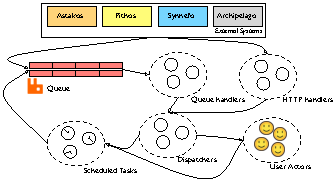
\includegraphics[scale=1.5]{arch.pdf}
    \end{center}
\caption{Functional components in Aquarium's architecture} 
\label{fig:arch}
\end{figure}

With event sourcing as the basis for Aquarium, we then proceeded to design the
system's runtime data model. What we wanted to model was the current state of
resource usage for each user, along with the user's wallet. One possibility we
wanted to explore on that front was copy on write updates; even for trivial
updates, the system would have to copy the affected data graphs to new
versions, instead of modifying the system in place. For that, we briefly
explored the use of software transactional memory, but found it restrictive for
our pursposes. What we chose instead was to contain each user's runtime state
in an actor. Using this design, shared state was eliminated; the use of the
actor model guarantee, that only one thread can execute within the context of
an actor renders the protection (with copy on write or other mechanism) of the
actor's state superflous. The actor model also fitted the event sourcing basis
very well, since each message in the log could pass through various processing
stages and reach the appropriate actor immutably.

\paragraph{Components} An overview of the Aquarium architecture is presented in
Figure~\ref{fig:arch}.  The system is modeled as a collection of logically and
functionally isolated components, which communicate by message passing. Withing
each component, a number of actors take care of concurrently processing
incoming messages through a load balancer component which is the gateway to
requests targeted to the component. Each component is also monitored by its own
supervisor; should an actor fail, the supervisor will automatically restart it.
The architecture allows certain application paths to fail individually while
the system is still responsive, while also enabling future distribution of
multiple components on clusters of machines.

The system receives input mainly from two sources: a queue for resource and
user events and a {\sc rest api} for billing state queries. The queue component
reads messages from a configurable number of queues and persists them in the
application's immutable log store. Both input components then forward incoming
messages to a network of dispatcher handlers which do not do any processing by
themselves, but know where the user actors lay. As described earlier, actual
processing of billing events is done within the user actors. Finally, a
separate network of actors take care of scheduling periodic tasks, such as
refiling of user credits; it does so by issuing events in the appropriate
queue.

\paragraph{Implementation}

Aquarium is being developed as a standalone service, based on the Akka library
for handling actor related functionality. Akka has all basic components for
implementing the architecture as described, which allowed us to focus on
implementing the business logic, leaving the details of actor registries,
dispatchers and message passing to Akka's runtime. Akka also provided
actor-based components for communicating with the message queue and, through a
third party component (Spray)\footnote{\url{http://github.com/spray}} for
handling {\sc rest} requests.  We chose the {\sc amqp} protocol and its
Rabbit{\sc mq} implementation for implementing the request queue, specifically
because recent versions include support for active/active cluster
configurations. The persistence layer is currently implemented by Mongo{\sc
db}, for its replication and sharding support.  However, this is not a hard
requirement, as Aquarium features an abstraction layer for all database queries
(currently 10 methods), which can then be implemented by any persistence
system, relational or not.


\section{Computational aspects}

%\subsection{Charging basics and cost policies}

In order to charge based on the incoming resource events, time (\DTime) and the unit of measure (\DUnitR) for a resource ($R$) play a central role. \DUnitR can be taken into account either as whole value or as a difference \DeltaDUnitR. On first approximation, these lead to linear formulas that capture the essence of charging algorithms. Below, we will briefly  study charging scenarios for three well-known resources, namely \textsf{bandwidth}, \textsf{diskspace} and \textsf{vmtime}. For the analysis of each case, we assume: 
\begin{itemize}
\item The arrival of two consecutive resource events, happening at times $t_0$ and $t_1$ respectively, with a time difference of  $\Delta T = \Delta T_{0, 1} = t_1 - t_0$.

\item The total values of resource $R$ for times $t_0$ and $t_1$ are $U_R^0$ and $U_R^1$ respectively.
%In general, for time $t_i$, the respective total value would be $U_R^i$.

\item The charging unit is denoted as $C$. %By definition it is one credit.

\item A factor in the form $[\frac{C}{D}]$ represents the resource-specific charging unit, where $C$ is defined above, and $D$ depends on the combination of the previously discussed dimensions ($T$, $U_R$) that enters the calculation. The meaning of the factor is probably clearer if we think of it as ``credits per $D$'', as the representation readily suggests.
\end{itemize}

\paragraph{\textsf{bandwidth}}
In this case, an event at $t_1$ records a change of bandwidth, using the relevant unit of measure $U_R$.  The credit usage computation is $\Delta U_R \cdot  [ \frac{C}{U_R} ]$.
A concrete example is $\Delta U_R = \MB{10}$ and in this case the bandwidth charging unit $[ \frac{C}{U_R} ]$ is ``$credits$ per {\sc MB}'', since $U_R$ is measured in {\sc MB}.

\paragraph{\textsf{diskspace}}
We take into account the disk space $U_R^0$ occupied at $t_0$ together with the time passed, $\Delta T$. The credit usage computation is $U_R^{0} \cdot \Delta T \cdot [ \frac{C}{U_R \cdot T} ]$.
That is, when we receive a new state change for disk space, we actually calculate for how long we occupied the total disk space without counting the new state change. If we had \GB{1} at $t_0 = \secs{1}$ and we gained another \GB{3.14} at $t_1 = \secs{3.5}$ then we are charged for the \GB{1} we occupied for $3.5 - 1 = 2.5$ seconds. The disk space charging unit $[ \frac{C}{U_R \cdot T} ]$ is ``$credits$ per {\sc GB} per $sec$'', assuming $U_R$ (disk space) is measured in {\sc GB} and time in $sec$.


\paragraph{\textsf{vmtime}}
Events for VM usage come into pairs that record \textsf{on} and \textsf{off} states of the VM. We use the time difference between these events for the credit usage computation, given by $\Delta T \cdot [ \frac{C}{T} ]$.


The charging algorithms for the sample resources given previously motivate related cost policies, namely \textsf{discrete}, \textsf{continuous} and \textsf{onoff}. Resources employing the \textsf{discrete} cost policy are charged just like \textsf{bandwidth}, those employing the \textsf{continuous} cost policy are charged like \textsf{diskspace} and finally resources with a \textsf{onoff} cost policy are charged like \textsf{vmtime}. Due to space limits we omit a more detailed analysis and the description of more involved scenarios.


%\subsection{State management}

%The only data mutation that takes place is the
%actor's state. Since each actor handles only its user's events and
%since there is only one actor for a user, the user state mutation is
%guaranteed to be race-free and events for different users are handled
%asynchronously and concurrently.

Scheduled tasks compute total charges, the updated resource state and
a total credit amount for each billing period. This computation is
recorded to a persistent store, in an append-only fashion, for future
reference and as a cached value. This cached value can be handy in
computations or in case of system crashes. In the latter, we wish to
avoid recomputation based on the whole history of events.

\section{Performance}

To evaluate the performance of Aquarium, we formulated an experiment
that evaluated two important properties: the time required to perform
the charging operation for a resource event and the overall time
required to process a resource event, end to end. To conduct the
experiment, Aquarium was configured, using the policy {\sc dsl} to
handle billing events for 5 types of resources, using 3 overloaded
pricelists, 2 overloaded algorithms, all of which were combined to 5
different agreements. Aquarium's data store was pre-filled in with
1.000.000 resource events, evenly distributed among 1.000 users. To
drive the benchmark, we used a synthetic load generator that produced
random billing events, at a configurable rate per minute.

To run the benchmark, we deployed Aquarium on a virtualized 4 core 2{\sc gh}z
class {\sc cpu} and 4{\sc gb} {\sc ram} Debian Linux server, on the Okeanos
cloud infrastructure. The virtual machine running Aquarium was configured with
a 4{\sc gb} maximum heap size.  Rabbit{\sc mq} and Mongo{\sc db} where run in
another 4-core, 4{\sc gb ram} virtual machine. The two virtual machines did not
share a physical host and communicated over Okeanos's switched network fabric
at an effective rate of 800 Mbits/sec, as reported by the \texttt{iperf}
utility. No
further optimization was performed on either back-end system.

\begin{figure}[t]
    \begin{center}
        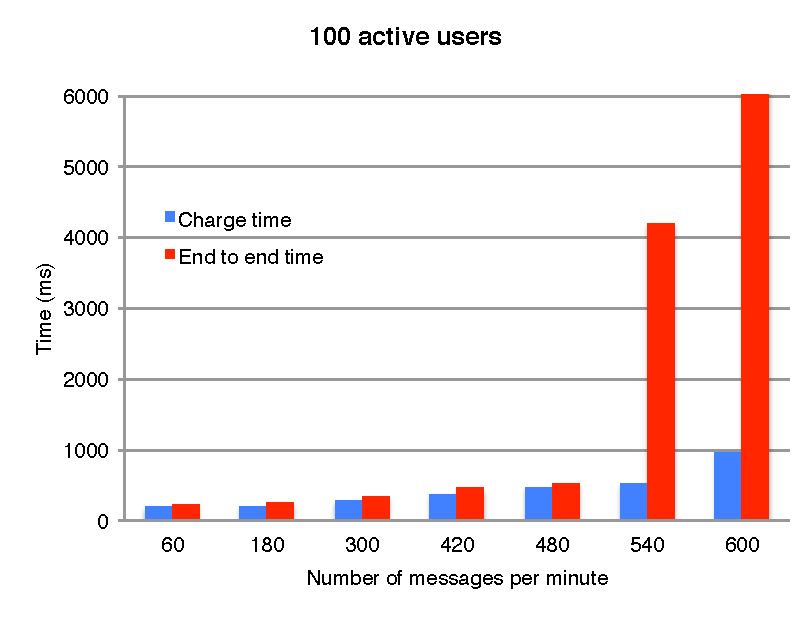
\includegraphics[scale=0.59]{perf.pdf}
    \end{center}

    \caption{Average time for performing a billing operation and end
      for end to end message processing for 100 active users and a
      varying number of messages per minute.}
    
    \label{fig:perf}
\end{figure}

All measurements were done using the first working version of the Aquarium
deployment, so no real optimisation effort has taken place. This shows in the
current performance measurements, as Aquarium was not able to handle more than
about 500 billing operations per second. One factor that contributed to this
result was the way resource state recalculations was done; in the current
version, the system needs to re-read parts of the event and billing state from
the datastore every time a new resource event appears. This contributes to more
than 50\% of the time required to produce a charging event, and can be
completely eliminated when proper billing snapshots are implemented. In other
measurements, we also observed that the rate of garbage creation was extremely
high, more that 250 {\sc mb}/sec. Upon further investigation, we attributed it
to the way policy timeslot applicability is calculated. Despite the high
allocation rate, the {\sc jvm}'s garbage collector never went through a
full collection cycle; when we forced one after the benchmark run was over, 
we observed that the actual heap memory usage was only 80{\sc mb}, which
amounts to less than 1 {\sc mb} per user.

% Even so, by extrapolating on the results and hardware configuration, an average
% 12-core box could handle more 1.500 messages per minute from about 300 active
% users, at 5 events per minute. Given that activity from users is expected to
% arrive in bursts, a more realistic expectation might be to receive 1 message
% per user per 5 minutes on average; in that case, and provided that the resource
% query cost is negligible as it is being served from an in memory cache, the
% system could handle around 4.500 concurrent users. While such back of the
% envelop calculations do not account for traffic spikes, they do provide an
% rough estimation of the optimisation effort that must be put in place. 

\section{Related Work}

Yousef et al.~\cite{Youse08} described the three pricing models that
are used by cloud service providers for billing used resources, namely
tiered pricing, per-unit pricing and subscription-based pricing.
Aquarium's cost policies that are assigned to resources map exactly to
Yousef's pricing models. In fact, most offerings by public IaaS
providers~\cite{Azure12, Amaz12} offer services charged according to
Yousef models.

Work on resource accounting and billing has been carried out in the
context cloud federation~\cite{Rochw09, Elmro09} and (earlier) grid
federation projects. The Distributed Grid Accounting System ({\sc
  dgas})~\cite{Piro06} was among the first to enable resource
accounting at the computing and storage layers and then aggregation of
the resources in a centralized location. The Reservoir project
investigated the use of service level agreements~\cite{Elmro09} for
resource provisioning in federated cloud scenarios.

On the cloud computing front, vendors such as VMWare, Microsoft and
{\sc ibm} provide full stack solutions, which also include resource
accounting. Usually, such systems are connected with existing
enterprise resource planning systems. \"Ubersmith has developed an
engine dedicated to resource accounting; much like Aquarium, it tracks
resource usage and applies accounting policies to it. On the open
source front, neither the Cloustack nor the Openstack projects, have
yet incorporated billing into their services. To the best of our
knowledge, Aquarium is the first open source system to offer
configurable accounting services for IaaS deployments.

%Check also~\cite{Ruiz-Agundez11}.

\section{Development Effort and Future Work}

A typesafe language was a hard requirement. Of the platforms examined,
the {\sc jvm} had the richest collection of ready made components; the
Akka library was particularly enticing for the scalability and
distribution possibilities it offered.

Scala as a language was an enabling factor; case classes permitted the
expression of data models, including the configuration {\sc dsl}, that
could be easily be serialized or read back from wire formats while
also promoting immutability through the use of the \texttt{copy()}
constructor. The pervasive use of immutability allowed us to write
strict, yet simple and concise unit tests, as the number of cases to
be examined was generally low. 

Akka's custom supervision hierarchies allowed us to partition the
system in self-healing sub-components, each of which can fail
independently of the other. For example, if the queue reader component
fails due to a queue failure, Aquarium will still be accessible and
responsive for the {\sc rest} interface. Also, Akka allowed us to
easily saturate the processing components of any system we tested
Aquarium on, simply by tuning the number of threads (in {\sc i/o}
bound parts) and actors (in {\sc cpu} bound parts) per dispatcher.

From a software engineering point of view, the current state of the project was
reached using about 8 person months of effort, 2 of which were devoted to
requirements elicitation, prototype building and familiarizing with the
language. The source code currently consists of 7.000 lines of executable
statements (including about 1.200 lines of tests), divided in about 10
packages. The system is built using both {\sc sbt} and Maven.

Aquarium is currenty under development, with a first production deployment
planned for April 2012. In the future, we plan to invest resources into
creating a comprehensive {\sc rest api} for accessing the user actor state and
to distribute the message processing accross multiple nodes in an active-active
mode.

\section{Acknowledgments and Availability}

Aquarium has been developed under contract from the Greek Ministry of Education
\todo{Fix Ack}

Aquarium is available under a {\sc bsd} 2-clause license from:
\url{https://code.grnet.gr/projects/aquarium}

{\footnotesize \bibliographystyle{acm}
\bibliography{aquarium}}

\theendnotes

\end{document}
